\documentclass{estilo}
\usepackage[spanish]{babel}
\usepackage{graphicx}
\usepackage{float}
\usepackage{amsmath}        % para los vectores columnas
\usepackage{amsfonts}       % para las negrita de pizarra
\usepackage{amssymb}        % para simbolos matematicos
\usepackage{hyperref}       % para utilizar referencias
\usepackage{multirow}       % para las tablas
\usepackage{dsfont}
\usepackage{listings}
\usepackage{xcolor}
\definecolor{codegreen}{rgb}{0,0.6,0}
\definecolor{codegray}{rgb}{0.5,0.5,0.5}
\definecolor{codepurple}{rgb}{0.58,0,0.82}
\definecolor{backcolour}{rgb}{0.95,0.95,0.92}
\lstdefinestyle{mystyle}{
    backgroundcolor=\color{backcolour},   
    commentstyle=\color{codegreen},
    keywordstyle=\color{magenta},
    numberstyle=\tiny\color{codegray},
    stringstyle=\color{codepurple},
    basicstyle=\ttfamily\footnotesize,
    breakatwhitespace=false,         
    breaklines=true,                 
    captionpos=b,                    
    keepspaces=true,                 
    numbers=left,                    
    numbersep=5pt,                  
    showspaces=false,                
    showstringspaces=false,
    showtabs=false,                  
    tabsize=2
}
\lstset{style=mystyle}

\usepackage{enumitem,multicol,setspace}
\newcounter{subenum}[enumi] % para las multicolumnas
\renewcommand{\thesubenum}{\arabic{subenum}}
\usepackage[nomessages]{fp}
\FPeval\thecolwidth{round(1/4:4)}% Specify number of columns -> column width
\newcommand{\newitem}[1]{%
  \refstepcounter{subenum}%
  \parbox{\dimexpr\thecolwidth\linewidth-.5\columnsep}{%
    \makebox[\labelwidth][r]{(\thesubenum)\hspace*{\labelsep}}%
    #1}\hfill%
}

\usepackage{scalerel,stackengine} % para el sombrero
\stackMath
\newcommand\rhat[1]{%
\savestack{\tmpbox}{\stretchto{%
  \scaleto{%
    \scalerel*[\widthof{\ensuremath{#1}}]{\kern-.6pt\bigwedge\kern-.6pt}%
    {\rule[-\textheight/2]{1ex}{\textheight}}%WIDTH-LIMITED BIG WEDGE
  }{\textheight}% 
}{0.5ex}}%
\stackon[1pt]{#1}{\tmpbox}%
}
\parskip 1ex

\usepackage{mathtools}      % floor y ceil
\DeclarePairedDelimiter\ceil{\lceil}{\rceil}
\DeclarePairedDelimiter\floor{\lfloor}{\rfloor} 

\usepackage[style=authoryear-comp]{biblatex}


\begin{document}
\maketitle

\justifying{}

%Tabla de contenidos
\newpage
\tableofcontents % Índice general
\newpage

\newpage
\section*{Consigna}


{\Large Introducción y primeros años}
\vskip0.5cm

Cuando Mateo nació, Sophia estaba muy contenta. Finalmente tendría un hermano con quien jugar. Sophi tenía 3 años cuando Mateo nació. Ya desde muy chicos, ella jugaba mucho con su hermano.

Pasaron los años, y fueron cambiando los juegos. Cuando Mateo cumplió 4 años, el padre de ambos le explicó un juego a Sophia: Se dispone una fila de $n$ monedas, de diferentes valores. En cada turno, un jugador debe elegir alguna moneda. Pero no puede elegir cualquiera: sólo puede elegir o bien la primera de la fila, o bien la última. Al elegirla, la remueve de la fila, y le toca luego al otro jugador, quien debe elegir otra moneda siguiendo la misma regla. Siguen agarrando monedas hasta que no quede ninguna. Quien gane será quien tenga el mayor valor acumulado (por sumatoria).

El problema es que Mateo es aún pequeño para entender cómo funciona esto, por lo que Sophia debe elegir las monedas por él. Digamos, Mateo está “jugando”. Aquí surge otro problema: Sophia es muy competitiva. Será buena hermana, pero no se va a dejar ganar (consideremos que tiene 7 nada más). Todo lo contrario. En la primaria aprendió algunas cosas sobre algoritmos greedy, y lo va a aplicar.
\vskip0.5cm
{\Large Consigna}
\vskip0.5cm

\begin{enumerate}
    \item Hacer un análisis del problema, y proponer un algoritmo greedy que obtenga la solución óptima al problema planteado: Dados los $n$ valores de todas las monedas, indicar qué monedas debe ir eligiendo Sophia para sí misma y para Mateo, de tal forma que se asegure de ganar siempre. Considerar que Sophia siempre comienza (para sí misma).
    \vskip0.3cm
    \item Demostrar que el algoritmo planteado obtiene siempre la solución óptima (desestimando el caso de una cantidad par de monedas de mismo valor, en cuyo caso siempre sería empate más allá de la estrategia de Sophia).
    \vskip0.3cm
    \item Escribir el algoritmo planteado. Describir y justificar la complejidad de dicho algoritmo. Analizar si (y cómo) afecta la variabilidad de los valores de las diferentes monedas a los tiempos del algoritmo planteado.
    \vskip0.3cm
    \item Analizar si (y cómo) afecta la variabilidad de los valores de las diferentes monedas a la optimalidad del algoritmo planteado.
    \vskip0.3cm
    \item Realizar ejemplos de ejecución para encontrar soluciones y corroborar lo encontrado. Adicionalmente, el curso proveerá con algunos casos particulares que deben cumplirse su optimalidad también.
    \vskip0.3cm
    \item Hacer mediciones de tiempos para corroborar la complejidad teórica indicada. Agregar los casos de prueba necesarios para dicha corroboración. Esta corroboración empírica debe realizarse confeccionando gráficos correspondientes, y utilizando la técnica de cuadrados mínimos. Para esto, proveemos una explicación detallada, en conjunto de ejemplos.
    \vskip0.3cm
    \item Agregar cualquier conclusión que les parezca relevante.
\end{enumerate}



\newpage

\justifying{
\hypertarget{res}{\section*{Resolución}}
\section{Ecuación de recurrencia}

A continuación se mostrará la \textbf{ecuación de recurrencia} hallada para este
problema:

\vskip0.5cm

\begin{center}
  
    $T(monedas, inicioFila, finFila) = \left\{ \begin{array}{lcc} K_{1} & si & K_{1} > K_{2} \\ \\ K_{2} & si & K_{1} < K_{2} \\  \end{array} \right.$

\end{center}

Siendo 

\vskip0.25cm

\begin{center}
  
    $K_{1} = monedas[inicioFila] + T(monedas, S(monedas, inicioFila + 1, finFila))$

    \vskip0.1cm
    $K_{2} = monedas[finFila] + T(monedas, S(monedas, inicioFila, finFila - 1))$
\end{center}


donde


$S(monedas, inicioFila, finFila) = \left\{ \begin{array}{lcc} (inicioFila+1,finFila) & si & monedas[inicioFila] > monedas[finFila] \\ \\ (inicioFila, finFila - 1) & si &  monedas[inicioFila] < monedas[finFila] \\  \end{array} \right.$

\vskip0.5cm

\textbf{NOTA}: 

$monedas$ = El vector con los valores de las monedas

$inicioFila$ = Es el valor de la primera moneda del vector monedas

$finFila$ = Es el valor de la última moneda del vector monedas

\vskip0.5cm

Nuestra función $T(monedas, inicioFila, finFila)$ nos otorga la ganancia que consiguió Sophia al momento de jugar con una cantidad de $n$ monedas contra Mateo. En esta, podemos observar como nuestras variables $K_{1}$ y $K_{2}$
realizan llamados recursivos a $T$ teniendo en cuenta como variables $inicioFila$ y $finFila$ la salida de otra función llamada $S(monedas, inicioFila, finFila)$ , que son las dos posibles decisiones que puede tomar mateo al elegir una moneda (recordemos que Mateo sigue una regla estricta de tomar la moneda de mayor valor entre la primera y la última).
\section{Demostración del Algortimo}

En un problema que involucra programacion dinamica, para hallar la solución óptima, o sea que nos de el \textbf{máximo valor acumulado posible}, se debe cumplir que:

\begin{enumerate}
    \item La solución óptima de un problema grande puede obtenerse combinando soluciones óptimas de subproblemas más pequeños.
    \item Esta descomposición debe hacerse de tal manera que no se omita ninguna posibilidad relevante para alcanzar la solución óptima.
    \item Se debe tomar una decisión sobre cuál subproblema o combinación de subproblemas proporciona el valor máximo.
\end{enumerate}

Vamos a demostrar entonces que nuestro algoritmo siempre encuentra la maxima ganancia que puede obtener Sophia:

\begin{itemize}
    \item Nuestro caso base es el siguiente: Si no hay monedas, Sophia tendría ganancia cero ya que no habría monedas para agarrar.
    \item Un subproblema es determinar la ganancia máxima que Sophia puede obtener en un intervalo de monedas dado por los índices \(i\) y \(j\) en el arreglo de monedas (donde \(i\) representa el índice de la primera moneda, y \(j\) el de la última). Para cada subproblema, Sophia debe tomar la decisión de sí:
    \begin{itemize}
        \item Agarrar la primera moneda \(m_i\), luego continuar con el subproblema de las monedas entre los índices \(i+2\) y \(j\) (si Mateo también agarró la primera moneda) o \(i+1\) y \(j-1\) (si Mateo agarró la última moneda).
        \item Agarrar la última moneda \(m_j\), luego continuar con el subproblema de las monedas entre los índices \(i+1\) y \(j-1\) (si Mateo agarró la primera moneda) o \(i\) y \(j-2\) (si Mateo también agarró la última moneda).
    \end{itemize}
    \item Como vemos en el ítem anterior, nuestros subproblemas cada vez se vuelven más pequeños, hasta eventualmente alcanzar el caso base (Top Down). A medida que vamos resolviendo los subproblemas, los memorizamos para no tener que recalcularlos, y ya que estamos considerando todas las posibilidades de decisión que puede tomar Sophia (y que va a tomar Mateo en consecuencia), hemos considerado (y memorizado) todas las soluciones a los subproblemas posibles, y con lo cual podemos hallar la solución óptima para nuestro problema original.
    \item Es decir, dado que cada subproblema se resuelve de forma óptima y se usan esas soluciones para construir la solución final, el algoritmo garantiza que dicha solución será la ganancia máxima que Sophia puede obtener.
\end{itemize}
\section{Algoritmo planteado y complejidad}

El algoritmo que decidimos utilizar para resolver el problema, es el siguiente:

\begin{verbatim}
    def juego_monedas(monedas):
    turno = 0 # Los turnos pares son de Sophia, los impares de Mateo
    i = 0
    j = len(monedas) - 1

    acum_sophia = 0
    acum_mateo = 0
    movimientos = []
    while not (i > j):
        primera_moneda = monedas[i]
        ultima_moneda = monedas[j]
        if turno % 2 == 0:
            if primera_moneda > ultima_moneda:
                acum_sophia += primera_moneda
                i += 1
                movimientos.append("Primera moneda para Sophia")
            else:
                acum_sophia += ultima_moneda
                j -= 1
                movimientos.append("Última moneda para Sophia")
        else:
            if primera_moneda < ultima_moneda:
                acum_mateo += primera_moneda
                i += 1
                movimientos.append("Primera moneda para Mateo")
            else:
                acum_mateo += ultima_moneda
                j -= 1
                movimientos.append("Última moneda para Mateo")
        turno += 1

    return movimientos, acum_sophia, acum_mateo
\end{verbatim}

\begin {itemize}
\item Mientras hayan monedas para elegir:
    \begin {itemize}
    \item Vemos las monedas que se encuentran en los dos extremos de la fila, y las comparamos:
        \begin {itemize}
        \item Si el turno es de Sophia, se elige la moneda de mayor valor.
        \item Si el turno es de Mateo, se elige la moneda de menor valor.
        \end {itemize}
    \end {itemize}
\item Devolvemos la ganancia acumulada de Sophia y Mateo.
\end {itemize}

Lo que estamos haciendo, es recorrer toda la fila de monedas (con dos índices, uno para cada extremo), y en cada iteración, comparamos las monedas, y acumulamos la ganancia para Sophia o Mateo (según corresponda el turno), y se agrega el movimiento que se realizó, hasta que finalmente ya no quedan monedas. Por lo tanto, siendo $n$ las monedas de la fila, nuestro algoritmo es lineal: O(n), ya que solamente recorremos ese arreglo de monedas, y en cada iteración hacemos operaciones de tiempo constante: O(1).

En conclusión, la complejidad algorítmica es: \textbf{O(n)}.
\section{Ejemplos de ejecución}
Se pueden encontrar encontrar multiples ejemplos de ejecución dentro del directorio \textit{ejemplos} en el repositorio. Veamos algunos:

Supongamos que tenemos 5 monedas:

\begin{lstlisting}
    [96, 594, 437, 674, 950]
\end{lstlisting}

En cada turno, Sophia tiene la opcion de elegir 2 monedas, la del principio o la del final. Esto implica que cada turno puede representarse como 2 opciones posibles, donde se debe elegir la opcion que acumule el mayor valor.

Para esto se recorren las opciones de manera recursiva, y se va seleccionando el maximo de los valores agregados en cada turno.

De esta forma, como se puede observar en el siguiente grafico, Sophia puede obtener un maximo de 1.483 puntos.

\begin{center}
    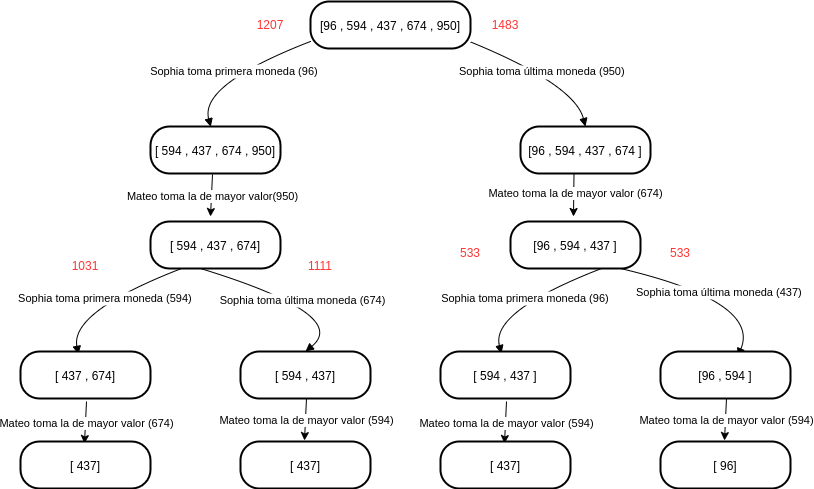
\includegraphics[scale = 0.5]{ {images/TDA-TP2.png} } 
\end{center}

Veamos lo que obtenemos al ejecutar en código el ejemplo que acabamos de ver:

\begin{center}
    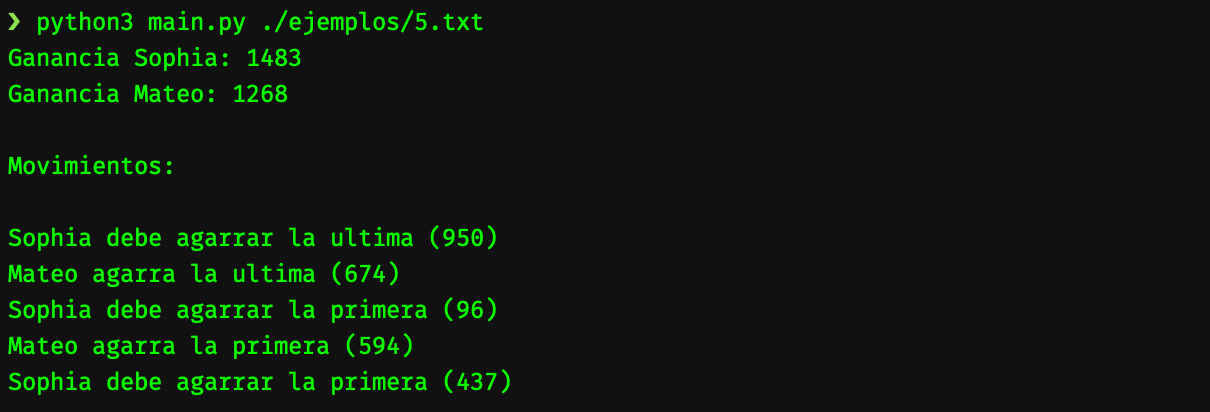
\includegraphics[scale = 0.6]{ {images/screen3.png} } 
\end{center}

Veamos la ejecución de otros ejemplos brindados por la cátedra:
\vskip0.5cm
Este ejemplo es con 10 monedas:
\begin{center}
    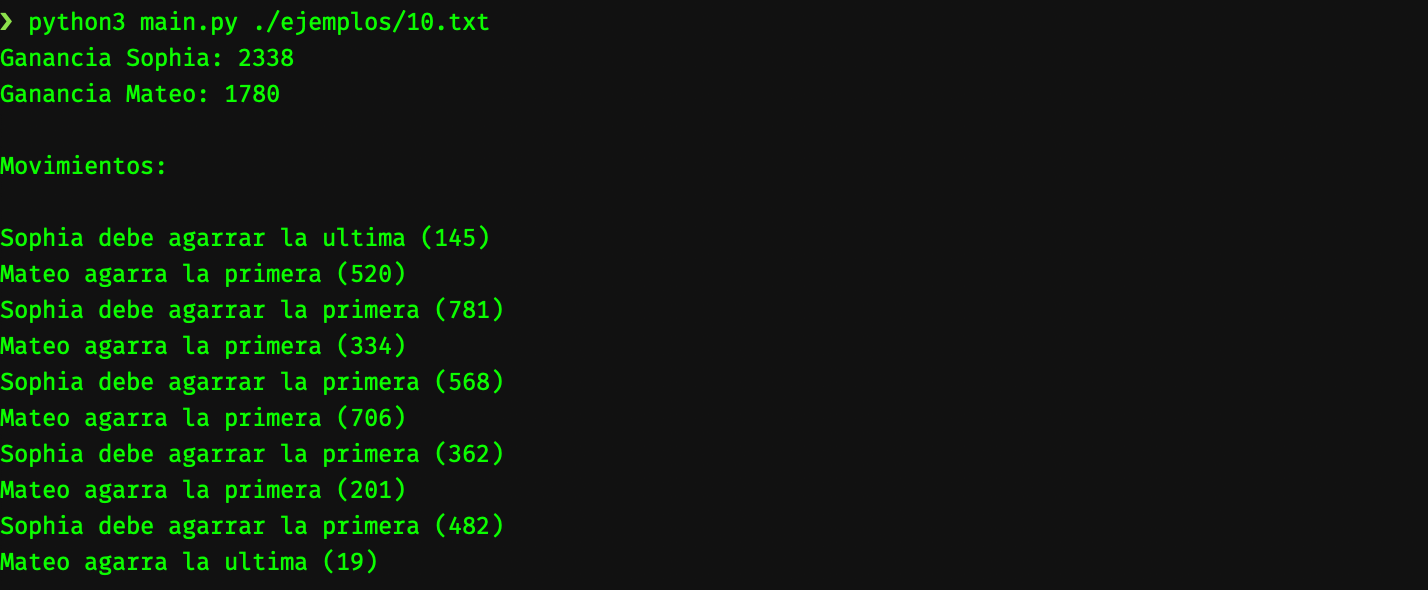
\includegraphics[scale = 0.6]{ {images/screen1.png} } 
\end{center}
Este ejemplo es con 25 monedas:
\begin{center}
    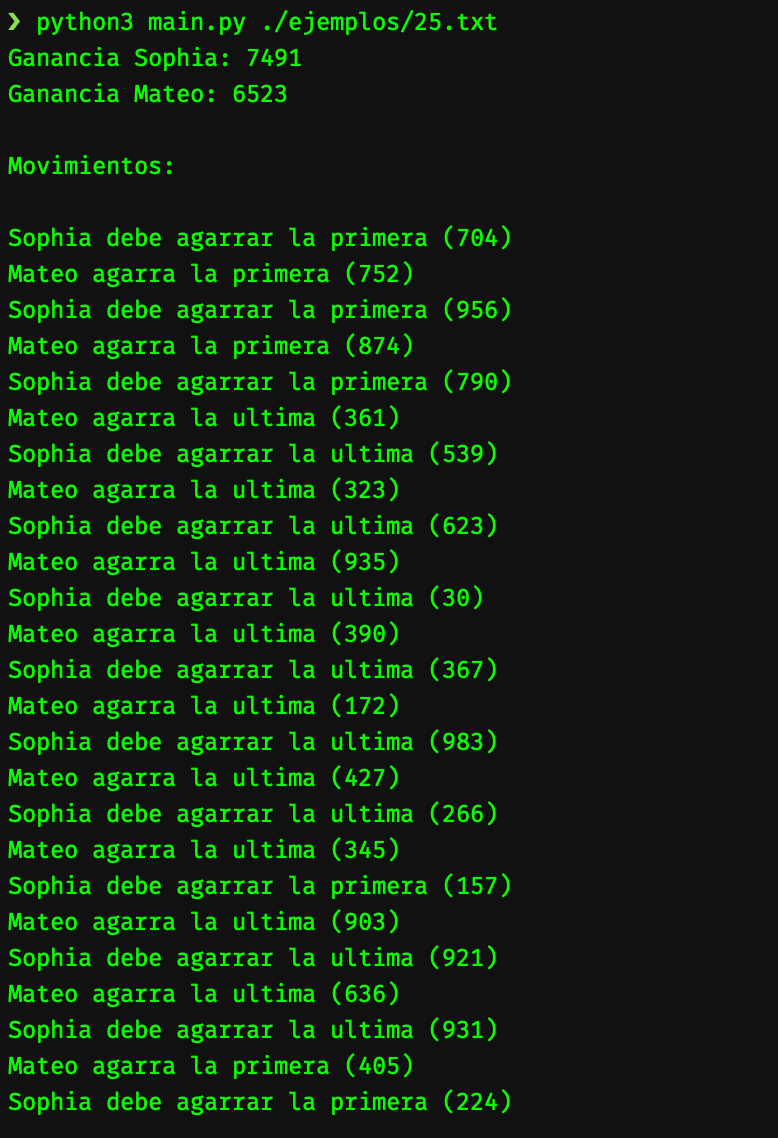
\includegraphics[scale = 0.6]{ {images/screen2.png} } 
\end{center}

Como podemos observar, los resultados obtenidos coinciden con los \textit{Resultados esperados} compartidos por la cátedra.

Ademas de estos ejemplos, se pueden encontrar otros en el directorio \textit{ejemplos} del repositorio. Los mismos pueden ser ejecutados con el comando \textit{pytest -v -s} en la terminal.

\begin{center}
    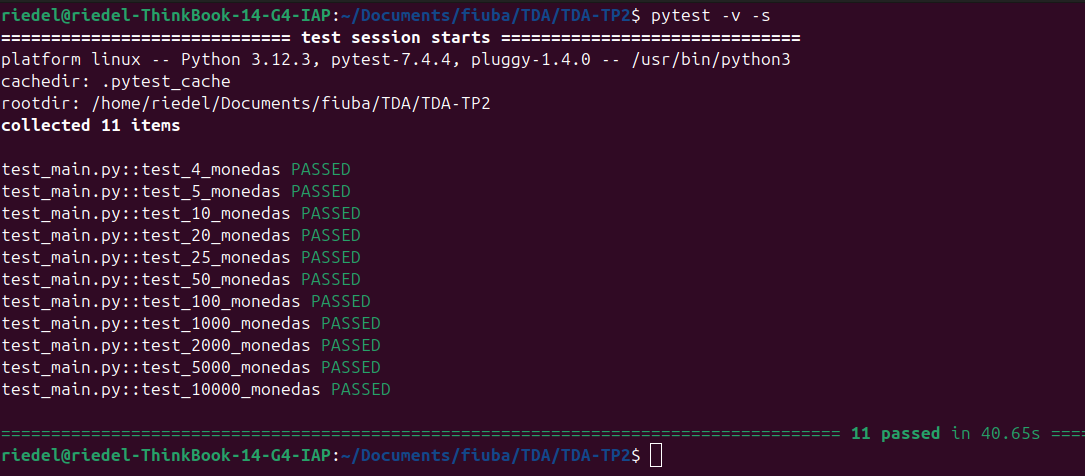
\includegraphics[scale = 0.4]{ {images/tests.png} } 
\end{center}
\section{Medición empírica}

Para comprobar empíricamente la complejidad \textbf{O($n^2$)} del algoritmo, se decidió ejecutar el mismo con distintos tamaños de entrada y medir el tiempo de ejecución. Se generaron muestras de tamaño n, las cuales varían desde 10 hasta 1000.

Para cada muestra se registró el tiempo de ejecución, obteniendo el siguiente gráfico:

\begin{center}
    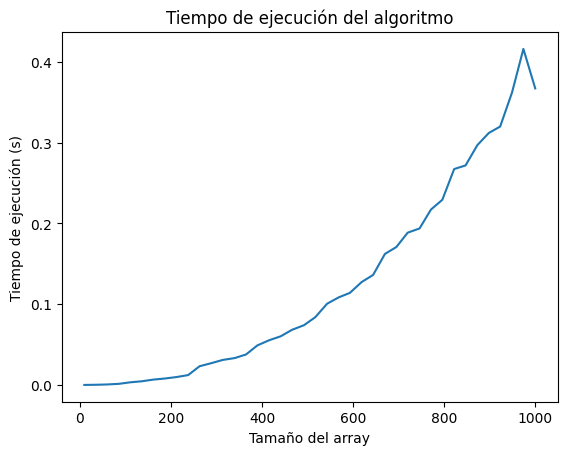
\includegraphics[scale = 0.6]{ {images/image.png} }
\end{center}


A simple vista se puede observar un crecimiento cuadratico. Para confirmar esto, vamos a ajustar los datos a una recta mediante cuadrados mínimos. Esto lo realizamos con Python y la función \textit{optimize.curve\_fit} de la biblioteca \textit{scipy}.


Obtenemos que el gráfico se puede ajustar a la curva $y = 4.86e^{-07}x^{2} -9.84e^{-05}x + 0.007$, con un error cuadrático medio de $9.37e^{-05}$. Por lo tanto, podemos verificar lo que ya vimos en la sección 3, que el orden es cuadratico \textbf{O($n^2$)}.

\begin{center}
    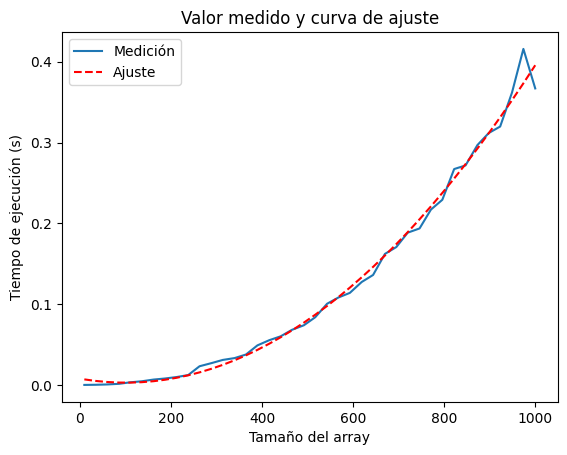
\includegraphics[scale = 0.6]{ {images/cuadradosMinimos.png} } 
\end{center}
\section{Conclusiones}

Pudimos observar y verificar lo siguiente:

\begin{itemize}

\item Utilizando la técnica de programación dinámica con memorización, pudimos reducir la complejidad de un algortimo exponencial a uno cuadrático, al no tener que recalcular problemas anteriormente resueltos.
\item Tras realizar un análisis empírico, pudimos confirmar que efectivamente la complejidad de nuestro algoritmo se vió beneficiada por la técnica de programación dinámica.
\item la variabilidad de los valores de las monedas \textbf{no} afecta en el tiempo de ejecución del algortimo.
\end {itemize}

En conclusión, el presente trabajo permitió afianzar los conocimientos adquiridos en la materia de una manera práctica, donde desarrollamos un algortimo con programación dinámica para resolver el problema planteado, con una complejidad cuadrática, obteniendo de esta manera la ganancia máxima que pudo haber adquirido Sophia.

}


\newpage
\end{document}